\section{Tests}


\subsection{test-1}

El test \texttt{test-1} se encarga de verificar la correctitud de las funciones \mintinline{c++}{void addAndInc(string key)}, \mintinline{c++}{bool member(string key)} y \mintinline{c++}{item maximum(unsigned int nt)}. En él se crea un \texttt{ConcurrentHashMap} y se agregan algunas palabras con \texttt{addAndInc}, verificando luego de cada llamado el valor de \texttt{member}. Para \texttt{maximum} se comprueba su valor usando un solo thread y también usando un cantidad de threads mayor a la cantidad de buckets.


\subsection{test-4}

En el test \texttt{test-4} se prueba la concurrencia de \texttt{addAndInc} creando varios threads que agregan palabras a un mismo \texttt{ConcurrentHashMap}, verificando la pertenencia al map con \texttt{member} y corroborando, una vez que terminan los threads, que \texttt{maximum} devuelve el valor correcto.


\subsection{test-6}

El test \texttt{test-6} tiene el objetivo de poner a prueba la concurrencia de las distintas funciones implementadas. Se crean varios threads que agregan palabras a un mapa propio y a otro mapa compartido por todos, usando distintas cantidades de threads para las funciones concurrentes como \texttt{count\_words} y \texttt{maximum}. La idea es tener una gran cantidad de threads corriendo concurrentemente para tratar de exponer errores. Al final se comprueba si es correcto el valor de \texttt{maximum} de cada uno de los mapas.


\subsection{test-7}

El fin de este test es comparar el tiempo de ejecución de las dos versiones de la función \mintinline{c++}{item maximum(unsigned int p_archivos, unsigned int p_maximos, list<string> archs)}: la que usa un mapa por thread y luego los combina en uno (\texttt{maximum}) y la que llama a \texttt{count\_words} (\texttt{maximum2}).

Se espera que \texttt{maximum} sea más lento que \texttt{maximum2} ya que el primero crea varios mapas que luego debe combinar, mientras que el segundo cuenta las palabras con sólo un mapa.

Para la prueba se ejecutaron las funciones para una lista de mil archivos, usando valores de \texttt{p\_archivos} y \texttt{p\_maximos} de 1 a 5.

En la figura \ref{fig:test_tiempos} se puede ver efectivamente que el tiempo de ejecución de \texttt{maximum} es mayor al de \texttt{maximum2} en todos los casos, llegando a ser más de 50\% más lento.

\begin{figure}[!h]
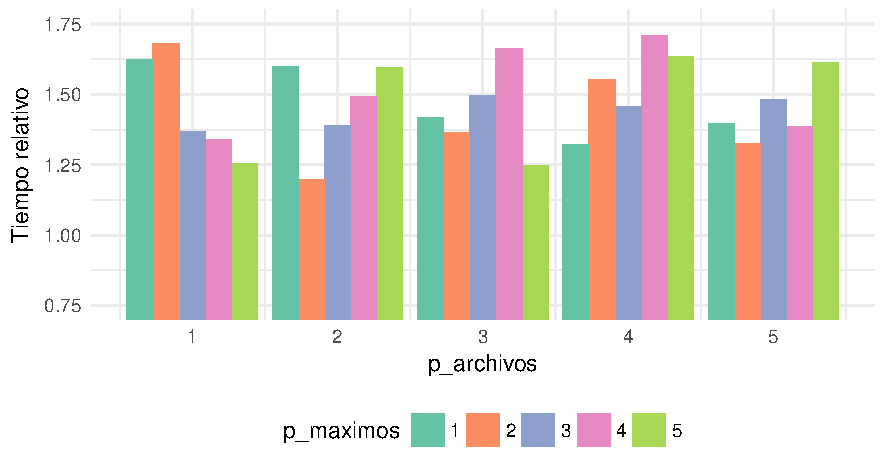
\includegraphics{figuras/tiempos.pdf}
\caption{Tiempo de \texttt{maximum} relativo al tiempo de \texttt{maximum2}}
\label{fig:test_tiempos}
\end{figure}


\subsection{test-8}

El test \texttt{test-8} tiene el objetivo de verificar si la función \mintinline{c++}{void addAndInc(string key)} implementa correctamente el mecanismo de locking que debería hacer exclusión mutua en caso de colisión únicamente.

Para hacer esto se crean dos listas de palabras de igual tamaño, cada una con una misma palabra repetida, pero que palabras de distintas las listas correspondan a buckets distintos (por ejemplo una lista \textless arbol, arbol, ..., arbol\textgreater\ y otra \textless bolso, bolso, ..., bolso\textgreater ). La razón por la cual se repite la misma palabra es que garantiza que \texttt{addAndInc} tenga un tiempo de ejecución constante.

Primero se crean dos threads que agregan la \emph{misma} la lista \emph{cada uno} a un \texttt{ConcurrentHashMap} y se mide el tiempo que demoran. Luego se crean otros dos threads que agregan cada uno una lista \emph{distinta} a un \texttt{ConcurrentHashMap} y se mide el tiempo que tarda. La idea es que cuando los dos threads agregan una misma lista el locking forzará un agregado secuencial; mientras que cuando agregan listas distintas los dos threads pueden agregar palabras concurrentemente ya que no hay colisión entre threads. Luego, los threads que agregan la misma lista deberían tardar mucho más.

Corriendo este test con listas de 100.000 palabras se obtuvo que los threads que agregan listas distintas demoran entre el 30\% y 34\% de lo que tardan los threads que agregan la misma lista. Esto confirma entonces que la implementación del locking es correcta.


\subsection{test-9}

Este test verifica que \mintinline{c++}{void addAndInc(string key)} y \mintinline{c++}{item maximum(unsigned int nt)} no sean concurrentes. Primero se carga un \texttt{ConcurrentHashMap} con palabras y se mide el tiempo que se tarda en llamar secuencialmente addAndInc y maximum una cierta cantidad de veces. Luego, se carga otro mapa con las mismas palabras y se mide el tiempo que se tarda en hacer lo mismo pero esta vez con dos threads, uno que llama a addAndInc y otro a maximum, la misma cantidad de veces. Se espera que los tiempos obtenidos sean aproximadamente el mismo.

El test dio como resultado que la ejecución con threads tarda entre 2\% y 5\% más que la ejecución secuencial. Este pequeño incremento puede atribuirse al overhead que conlleva el uso de threads. Con esto se comprueba entonces que las dos funciones no son concurrentes.


